\chapter{AnacondaによるPython開発環境の構築(補足)\label{chap:anaconda}}
ここではPythonの数値計算ライブラリ一式と、対話的実行環境であるJupyter-notebookを含むパッケージであるAnacondaのダウンロード・インストール方法について述べる。
PythonやJupyterは現在は京都大学の教育用教PC端末で用いることができるが、
各自のPCにもインストールしておくことを勧める。

本章ではWindowsへのインストール方法を述べるが、OS XやLinux等で用いる場合は

\url{https://www.continuum.io/downloads}

\noindent を参考にすること。

\section{Anacondaのダウンロード}
Anacondは無料かつオープンソース(ソースコードが公開されていること)のソフトウェアであり

\url{https://www.continuum.io/downloads}

\noindent から自由にダウンロードできる。

Windowsにインストールする場合は、図\ref{fig:Anaconda_download}にあるように、Windows用のものをダウンロードする。
Pythonにはバージョン2系統のものと3系統のものがあるが、
最新のものである3系統のもの(図ではPython3.5)をダウンロードすること。


\begin{figure}
	\centering
	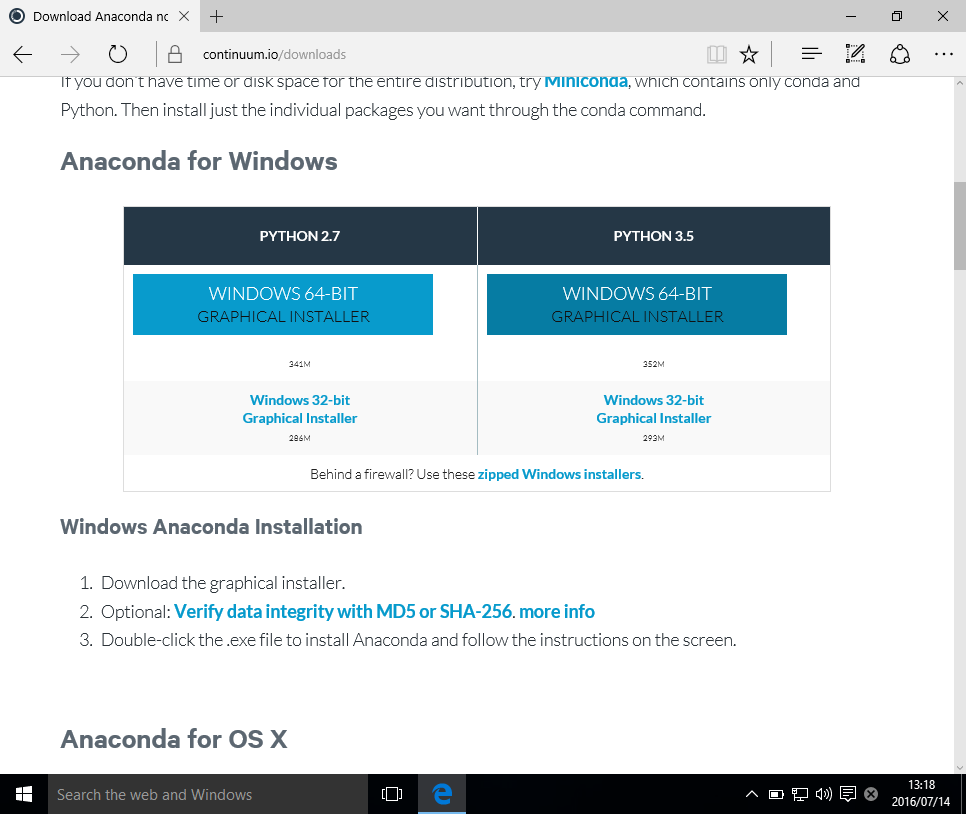
\includegraphics[width=10cm]{TeX_files/fig_python_install/Anaconda_download.png}
	\caption{
		\label{fig:Anaconda_download}
		Anacondaのダウンロードページの様子。Windows用のPython3.5のものをダウンロードすること。
	}
\end{figure}


\section{Anacondaのインストール}
先ほどダウンロードしたファイルを実行(クリック)することでインストールが始まる。

ダウンロードしたファイルの保存場所がわからなければインターネットブラウザの設定を確認する。
多くの場合、デフォルトではダウンロードフォルダ(図\ref{fig:Anaconda_install1}参照)にダウンロードされる。

インストーラにはいくつか質問されるが、よくわからなければデフォルトのままでよい。

\begin{figure}
	\centering
	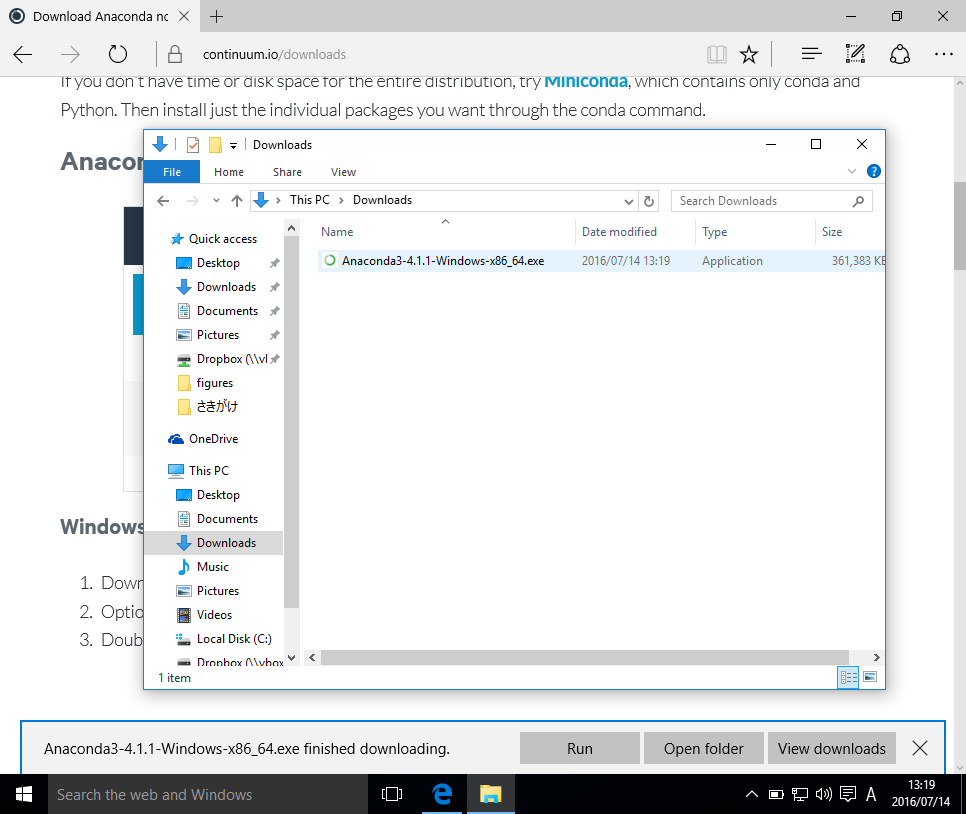
\includegraphics[width=10cm]{TeX_files/fig_python_install/Anaconda_install.png}
	\caption{
		\label{fig:Anaconda_install1}
		ダウンロードした場所をエクスプローラで開き、ファイルを実行する。
	}
\end{figure}

\begin{figure}
	\centering
	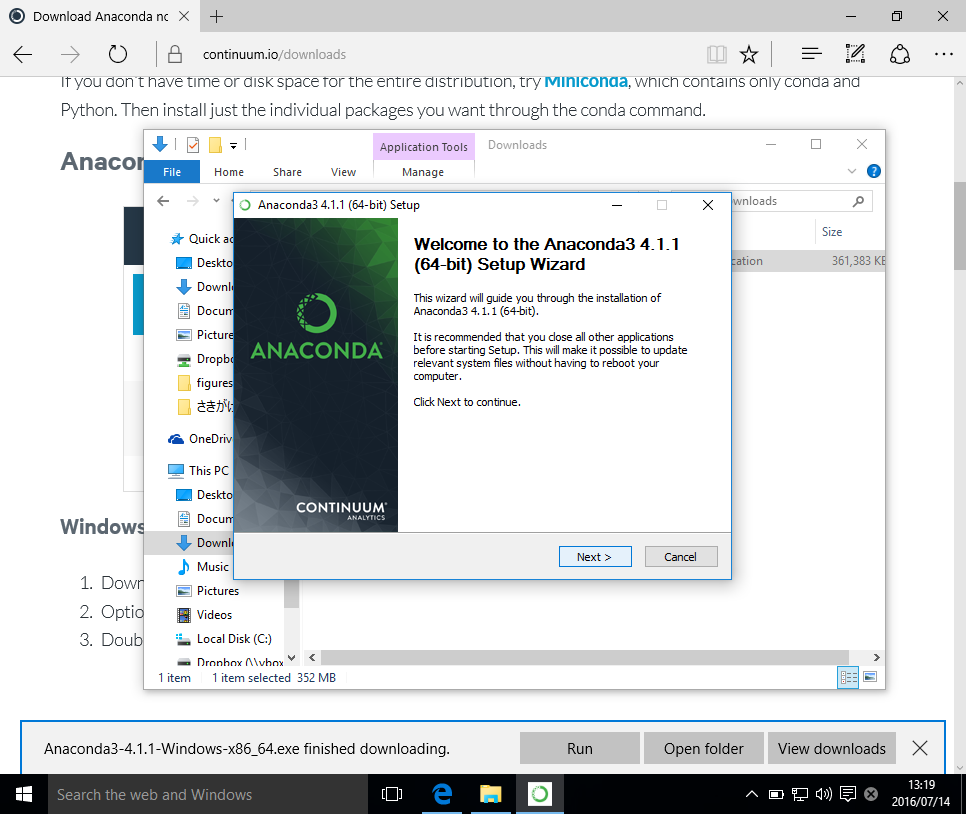
\includegraphics[width=10cm]{TeX_files/fig_python_install/Anaconda_install2.png}
	\caption{
		\label{fig:Anaconda_install2}
		インストーラを実行した時の様子。
	}
\end{figure}

\begin{figure}
	\centering
	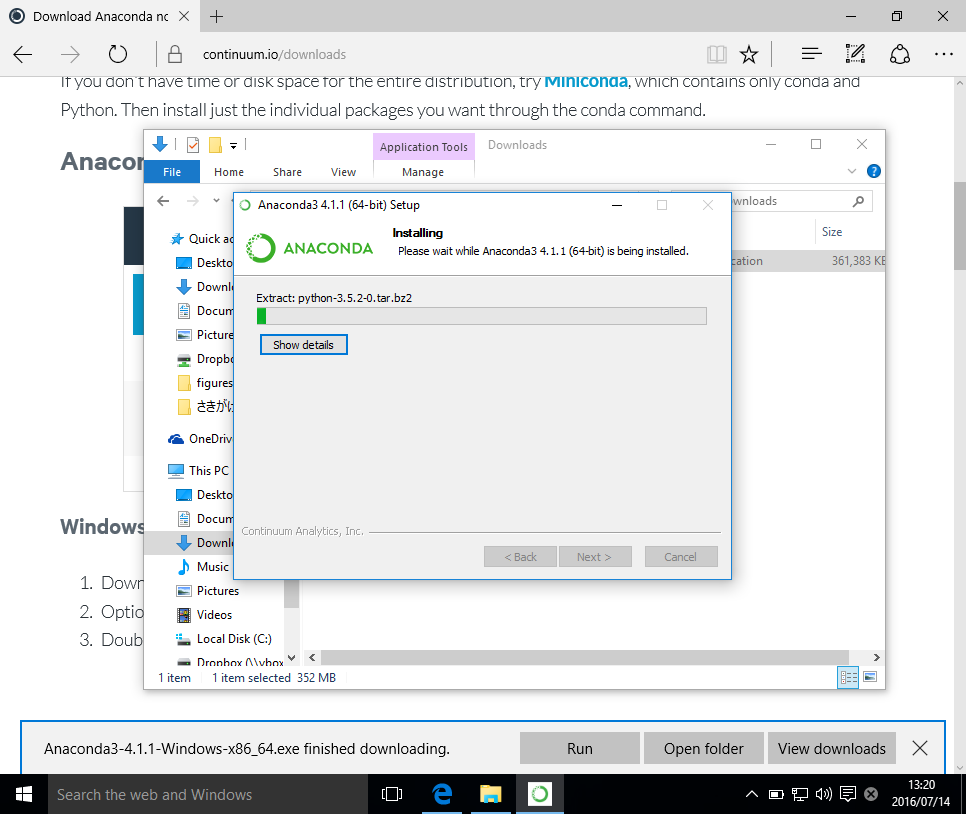
\includegraphics[width=10cm]{TeX_files/fig_python_install/Anaconda_install3.png}
	\caption{
		\label{fig:Anaconda_install3}
		インストールには少し時間がかかる。
	}
\end{figure}

\begin{figure}
	\centering
	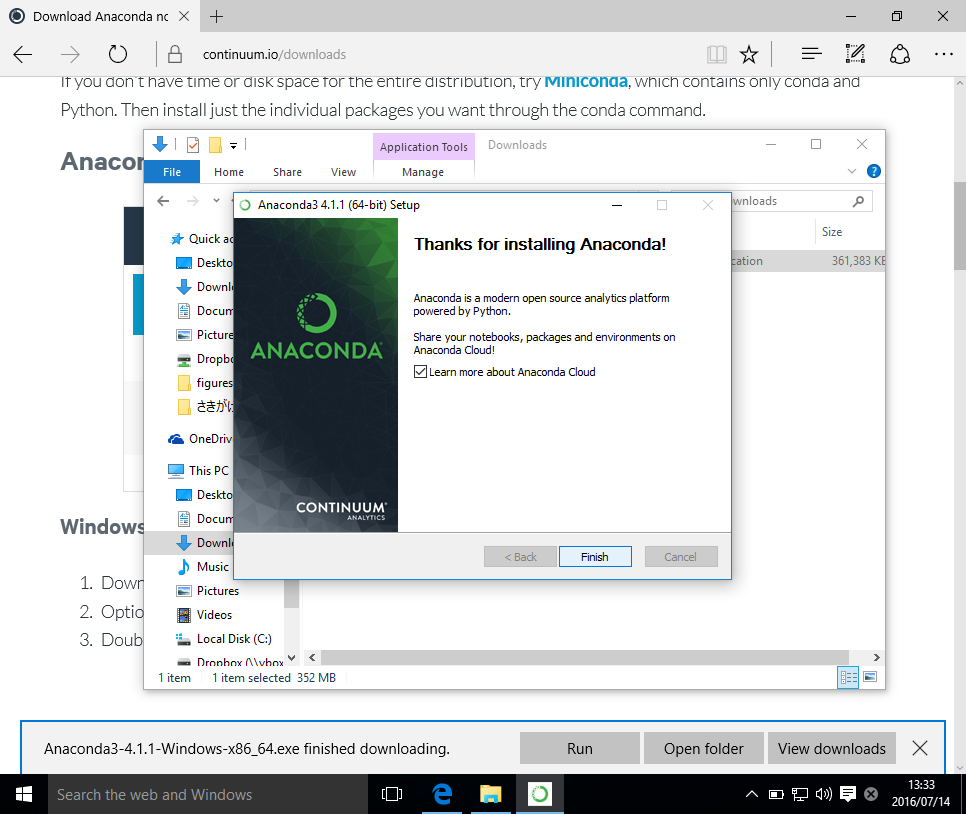
\includegraphics[width=10cm]{TeX_files/fig_python_install/Anaconda_install5.png}
	\caption{
		\label{fig:Anaconda_install5}
		このような画面が出れば完成である。
	}
\end{figure}
